% Chapter Template

\chapter{Ensayos y resultados} % Main chapter title
En este capítulo se detallan los ensayos realizados en las formaciones ferroviarias y en los talleres de Trenes Argentinos. El orden cronológico de los ensayos es distinto al del desarrollo del firmware. En este documento se ha presentado previamente el diseño de la solución para facilitar la comprensión del trabajo realizado. El desarrollo de la solución fue posterior a una serie de mediciones realizadas en los talleres que permitieron identificar parámetros clave del sistema. \\

En las secciones que siguen se explican las mediciones realizadas en las visitas a los talleres de Victoria y Castelar de Trenes Argentinos Operaciones. Luego se presenta un análisis de datos de las tramas relevadas y también las pruebas de integración propuestas para validar el desarrollo. \\


\label{Chapter4} % Change X to a consecutive number; for referencing this chapter elsewhere, use \ref{ChapterX}

%----------------------------------------------------------------------------------------
%	SECTION 1
%----------------------------------------------------------------------------------------
\section{Ensayos en trenes}

Uno de los objetivos generales del proyecto en el que se enmarcó este trabajo, era relevar las soluciones existentes de la red TCN y PIDS. A lo largo del desarrollo, se realizaron reuniones de trabajo con el personal de Trenes Argentinos Operaciones, y visitas a los talleres de la Gerencia de material rodante eléctrico para relevar información técnica. En orden cronológico, incluyendo trabajo realizado en etapa de confinamiento por COVID-19, se resaltan las siguientes interacciones con SOFSE:\\


\begin{enumerate}

\item 2020-05-20: se ensayaron mediciones sobre la maqueta de los talleres de Castelar, coordinadas de forma remota, para obtener mediciones de datos de la red RS485 del sistema PIDS.

\item 2020-06-30: se ensayaron mediciones sobre formaciones ferroviarias operativas en los talleres de Victoria, relevando los puntos de interconexión de la red TCN con el TLCD (pantalla táctil del conductor). Se realizaron también mediciones en el punto de interconexión del bus MVB con el módulo RCMe. 

\item 2020-09-23: se ensayaron nuevas mediciones, coordinadas de forma remota, en la maqueta de Castelar con un nuevo módulo analizador de datos.

\item 2021-04-09: se relevaron los puntos de interconexión entre RCMe y el PIDS, y entre los módulos IDU y SCU en formaciones operativas en los talleres de Victoria. También se ensayaron mediciones sobre el bus de datos RS485 que conecta el SCU con la DACU.

\item 2021-06-04: se ensambló una maqueta local usando un cartel led compatible con la serie de los carteles de trenes relevados y se presentó como informe de avance.

\item 2022-08-11, CASE 2022.

\end{enumerate}


En la figura \ref{fig:maquetaCastelar} se muestra la maqueta instalada en los talleres de Castelar. Se puede observar un rack con los módulos del sistema PIDS, incluyendo la pantalla LCD táctil que maneja el conductor. También se observan los carteles de matriz led frontal (cartel grande), de salón (cartel chico) y el mapa led con el recorrido de las estaciones (cartel del medio).\\
 
\begin{figure}[H]
	\centering
	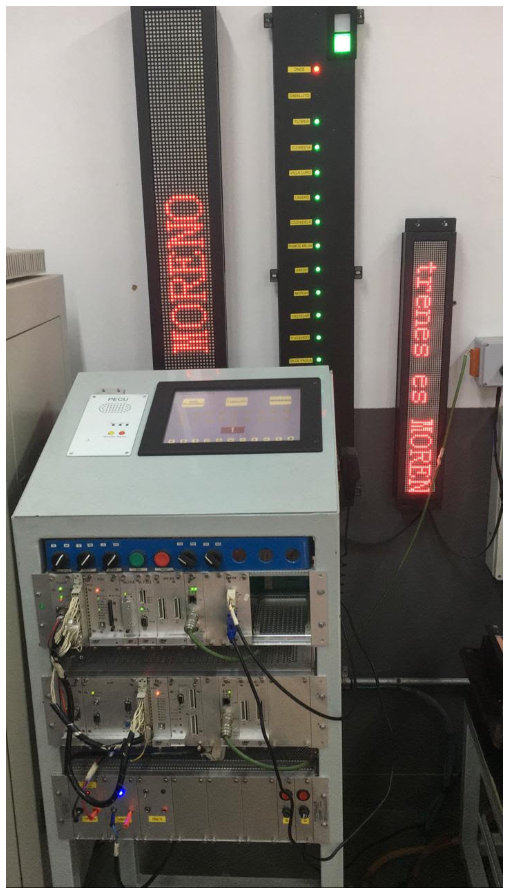
\includegraphics[width=0.66\textwidth]{./Figures/maqueta.png}
	\caption{Maqueta en talleres de Castelar.}
	\label{fig:maquetaCastelar}
\end{figure}


Durante las visitas a los talleres de Victoria, se pudo acceder a los planos eléctricos del sistema de comunicaciones del tren. Esta información resultó muy relevante ya que permitió comprender la lógica de interconexión de los módulos del tren y preparar un sistema de medición. Como consecuencia de las visitas, se fueron desarrollando piezas sueltas de hardware para realizar mediciones in-situ, a partir del relevamiento de los conectores y conexiones entre módulos.\\


Las redes del sistema PIDS y TCN siguen el estándar RS-485. Este tipo de redes es muy utilizada para transmisión y recepción de datos, ya que tiene interfaces eléctricas muy robustas que usan señales diferenciales, y que normalmente se implementan en cables de par trenzado, permitiendo cableados largos con buena inmunidad al ruido eléctrico. \\

En las figuras \ref{fig:conexionOriginal} y \ref{fig:conexionIntervenida} se presenta un diagrama esquemático del punto de medición y una fotografía de la medición realizada en el sitio, esto es, en una formación operativa en los talleres de Victoria. La conexión original muestra un grupo de tres cables nomenclados como 4330a, 4330b y 4330s, que corresponden con las líneas del bus RS485, RS485a, RS485b y RS485c respectivamente, que conecta el SCU con la placa (IDU) de la placa de control del cartel de matriz led.  La intervención en el punto de medición se realizó a través de una placa fabricada ad-hoc. Esta placa cuenta con conectores Harting de entrada y salida, facilitados por el personal de SOFSE, conversores RS485-USB y un analizador lógico programable, utilizado para decodificar en tiempo real los datos medidos.\\



\begin{figure}[H]
	\centering
      \includegraphics[width=0.25\textwidth]{./Figures/conexionOriginal.png}
      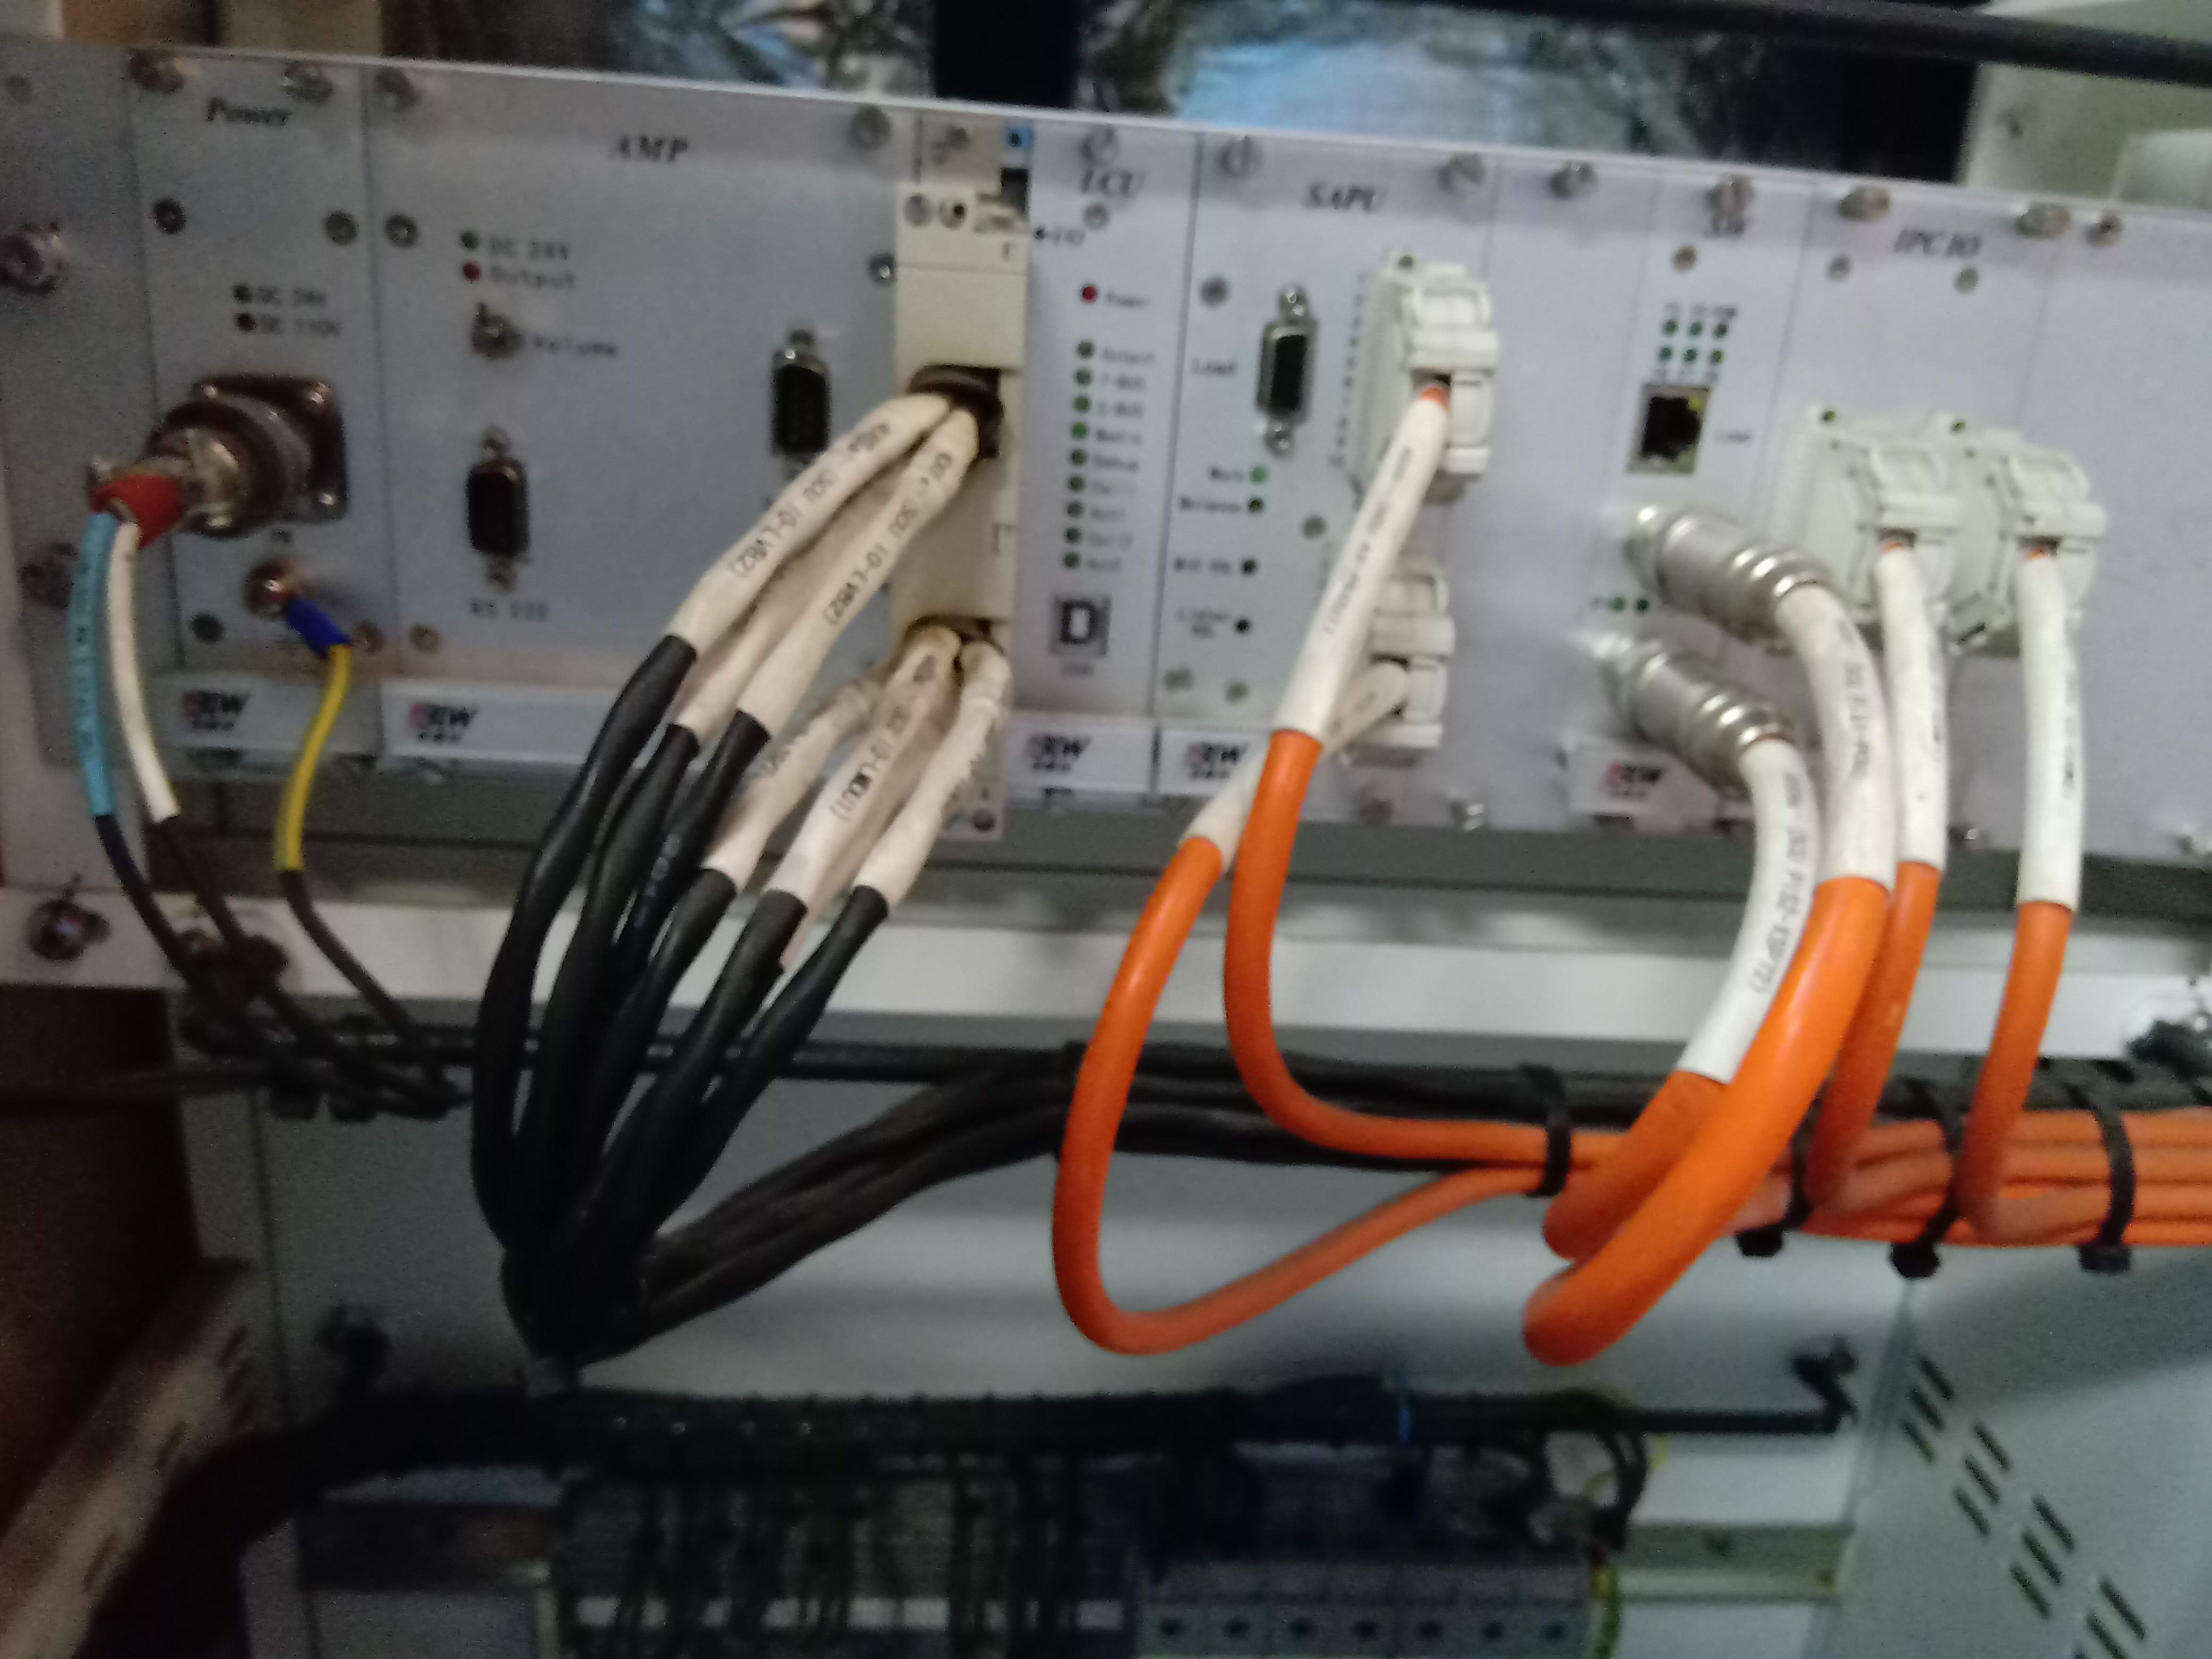
\includegraphics[width=0.5\textwidth]{./Figures/rackPIDS2.jpg}
	\caption{Diagrama esquemático y fotografía del punto de medición en la conexión SCU-IDU.}
	\label{fig:conexionOriginal}
\end{figure}

\begin{figure}[H]
	\centering
      \includegraphics[width=0.4\textwidth]{./Figures/conexionIntervenida.png}
      \includegraphics[width=0.5\textwidth]{./Figures/setupExperimentalMediciones.jpg}
	\caption{Diagrama esquemático y fotografía de la intervención para realizar mediciones en la conexión SCU-IDU.}
	\label{fig:conexionIntervenida}
\end{figure}




\begin{figure}[H]
	\centering
	\includegraphics[width=0.66\textwidth]{./Figures/sniffer.jpg}
	\caption{Pieza de hardware desarrollada ad-hoc para realizar mediciones.}
	\label{fig:sniffer}
\end{figure}




\begin{figure}[H]
	\centering
	\includegraphics[width=1\textwidth]{./Figures/medicionesVictoria2.png}
	\caption{Fotos de la jornada de mediciones en los talleres de Victoria.}
	\label{fig:medicionesVictoria2}
\end{figure}

La figura \ref{fig:placa} muestra una fotografía del hardware de control de los carteles de matriz led de Trenes Argentinos. Esta placa fue revisada en detalle y se han relevado los siguientes bloques de control:
\begin{itemize}
\item Conector de entrada del bus RS485.
\item Módulos de conversión de tensión.
\item Circuito de optoacopladores para las señales de datos.
\item Microcontrolados y circuito lógico.
\item Conector de salida para el cartel de matriz led.
\item Conector de programación.
\end{itemize}

El circuito eléctrico completo de esta placa ha sido relevado y se puede encontrar en el apéndice. Su función principal es la de decodificar las señales del tren y transmitir los mensajes al cartel de matriz led. El bloque de conversión de tensión contiene varios módulos, que son fuentes conmutadas para transformar la tensión de línea del tren de 110 Volt de corriente contínua en tensiones compatibles con el circuito de datos, por ejemplo 5 Volt o 3,3 Volt.\\

En la figura \ref{fig:mediciones} se muestra una fotografía del banco de medición operando en vivo en una de las formaciones ferroviaras operativas en los talleres de Victoria. Se puede observar la pieza de hardware desarrollada conectada al SCU de un lado, y a la laptop del otro. En la pantalla de la computadora se observan las líneas de datos capturadas por el analizador lógico programable.\\

\begin{figure}[H]
	\centering
	\includegraphics[width=0.66\textwidth]{./Figures/mediciones.jpg}
	\caption{Foto del banco de prueba midiendo en vivo en los talleres de Victoria.}
	\label{fig:mediciones}
\end{figure}



Según la topología de la red PIDS vista, los buses de datos siguen un esquema de tres cables por bus, nomenclados como RS485-A, RS485-B y RS485-C. En particular, la conexión entre el módulo SCU y los carteles de matriz led es por medio del bloque IDU, con los cables 4330a, 4330b y 4330c, números que corresponden al cableado físico. La conexión del SCU al IDU está incluída en un conector Harting de 48 pines, donde se unen varios buses o cableados RS485 de tres líneas.  \\

Los carteles de salón están embebidos en un gabinete de metal, donde se aloja la placa de control y parte del cableado. Esta placa de control
 
\section{Análisis de mediciones}

Los datos relevados en las sucesivas mediciones realizadas han aportado información.\\
Se ha obtenido información acerca del contenido de las tramas para la comunicación entre los sistemas TCMS-PIDS. La información de las tramas que el se detalla con el diagrama de la figura \ref{fig:tramasHeaderPayload}


\begin{figure}[H]
	\centering
	\includegraphics[width=1\textwidth]{./Figures/tramasHeaderPayload.png}
	\caption{Contenido de las tramas de datos entre TCMS y PIDS.}
	\label{fig:tramasHeaderPayload}
\end{figure}

En la figura \ref{fig:tramasBitsIDU} se detalla el contenido de los bytes en la comunicación con dirección PIDS-TCMS. Estas son tramas de longitud mucho mayor a las que se dan en el sentido inverso TCMS-PIDS. Se puede observar que los bits de cada byte están referidos a dispositivos específicos del sistema. Se ha resaltado en color los bits que corresponden a los módulos IDU, y que se puede observar según la nomenclatura que existen hasta 18 unidades de estos módulos, agrupados de a pares por cada salón. Son estos bits los que aportan información acerca del estado de los carteles de matriz led de salón.\\


\begin{figure}[H]
	\centering
	\includegraphics[width=1\textwidth]{./Figures/tramasBitsIDU.png}
	\caption{Detalle bit a bit de los bytes con contenido para el PIDS.}
	\label{fig:tramasBitsIDU}
\end{figure}



\begin{figure}[H]
	\centering
	\includegraphics[width=0.5\textwidth]{./Figures/logFile.png}
	\caption{Detalle de mediciones registradas en formato hexadecimal.}
	\label{fig:logFile}
\end{figure}


\begin{itemize}
\item 7EDFFFFFDEEFBFFFBFF7E
\item 7EBDFFFF7FFFFFFFFFFFFFFF39F7E
\item 7EBDFFFF7FFFFFFFFFFFFFFF39F7E
\item 7EBDFFFF7FFFFFFFFFFFFFFF39F7E
\item 7EFFFF7FFFFFFFFFFFFFEFFFA317E
\item 7E19ABF5FFFFFFFFFFFFFFFFFF7F72A85AF7E
\item 7E7CB12914AEDFFFFFFFEFFEFFBFFFFFF7F7FFFFFFFFFDFFFFB77E
\end{itemize}



\section{Hardware existente}

\begin{figure}[H]
	\centering
	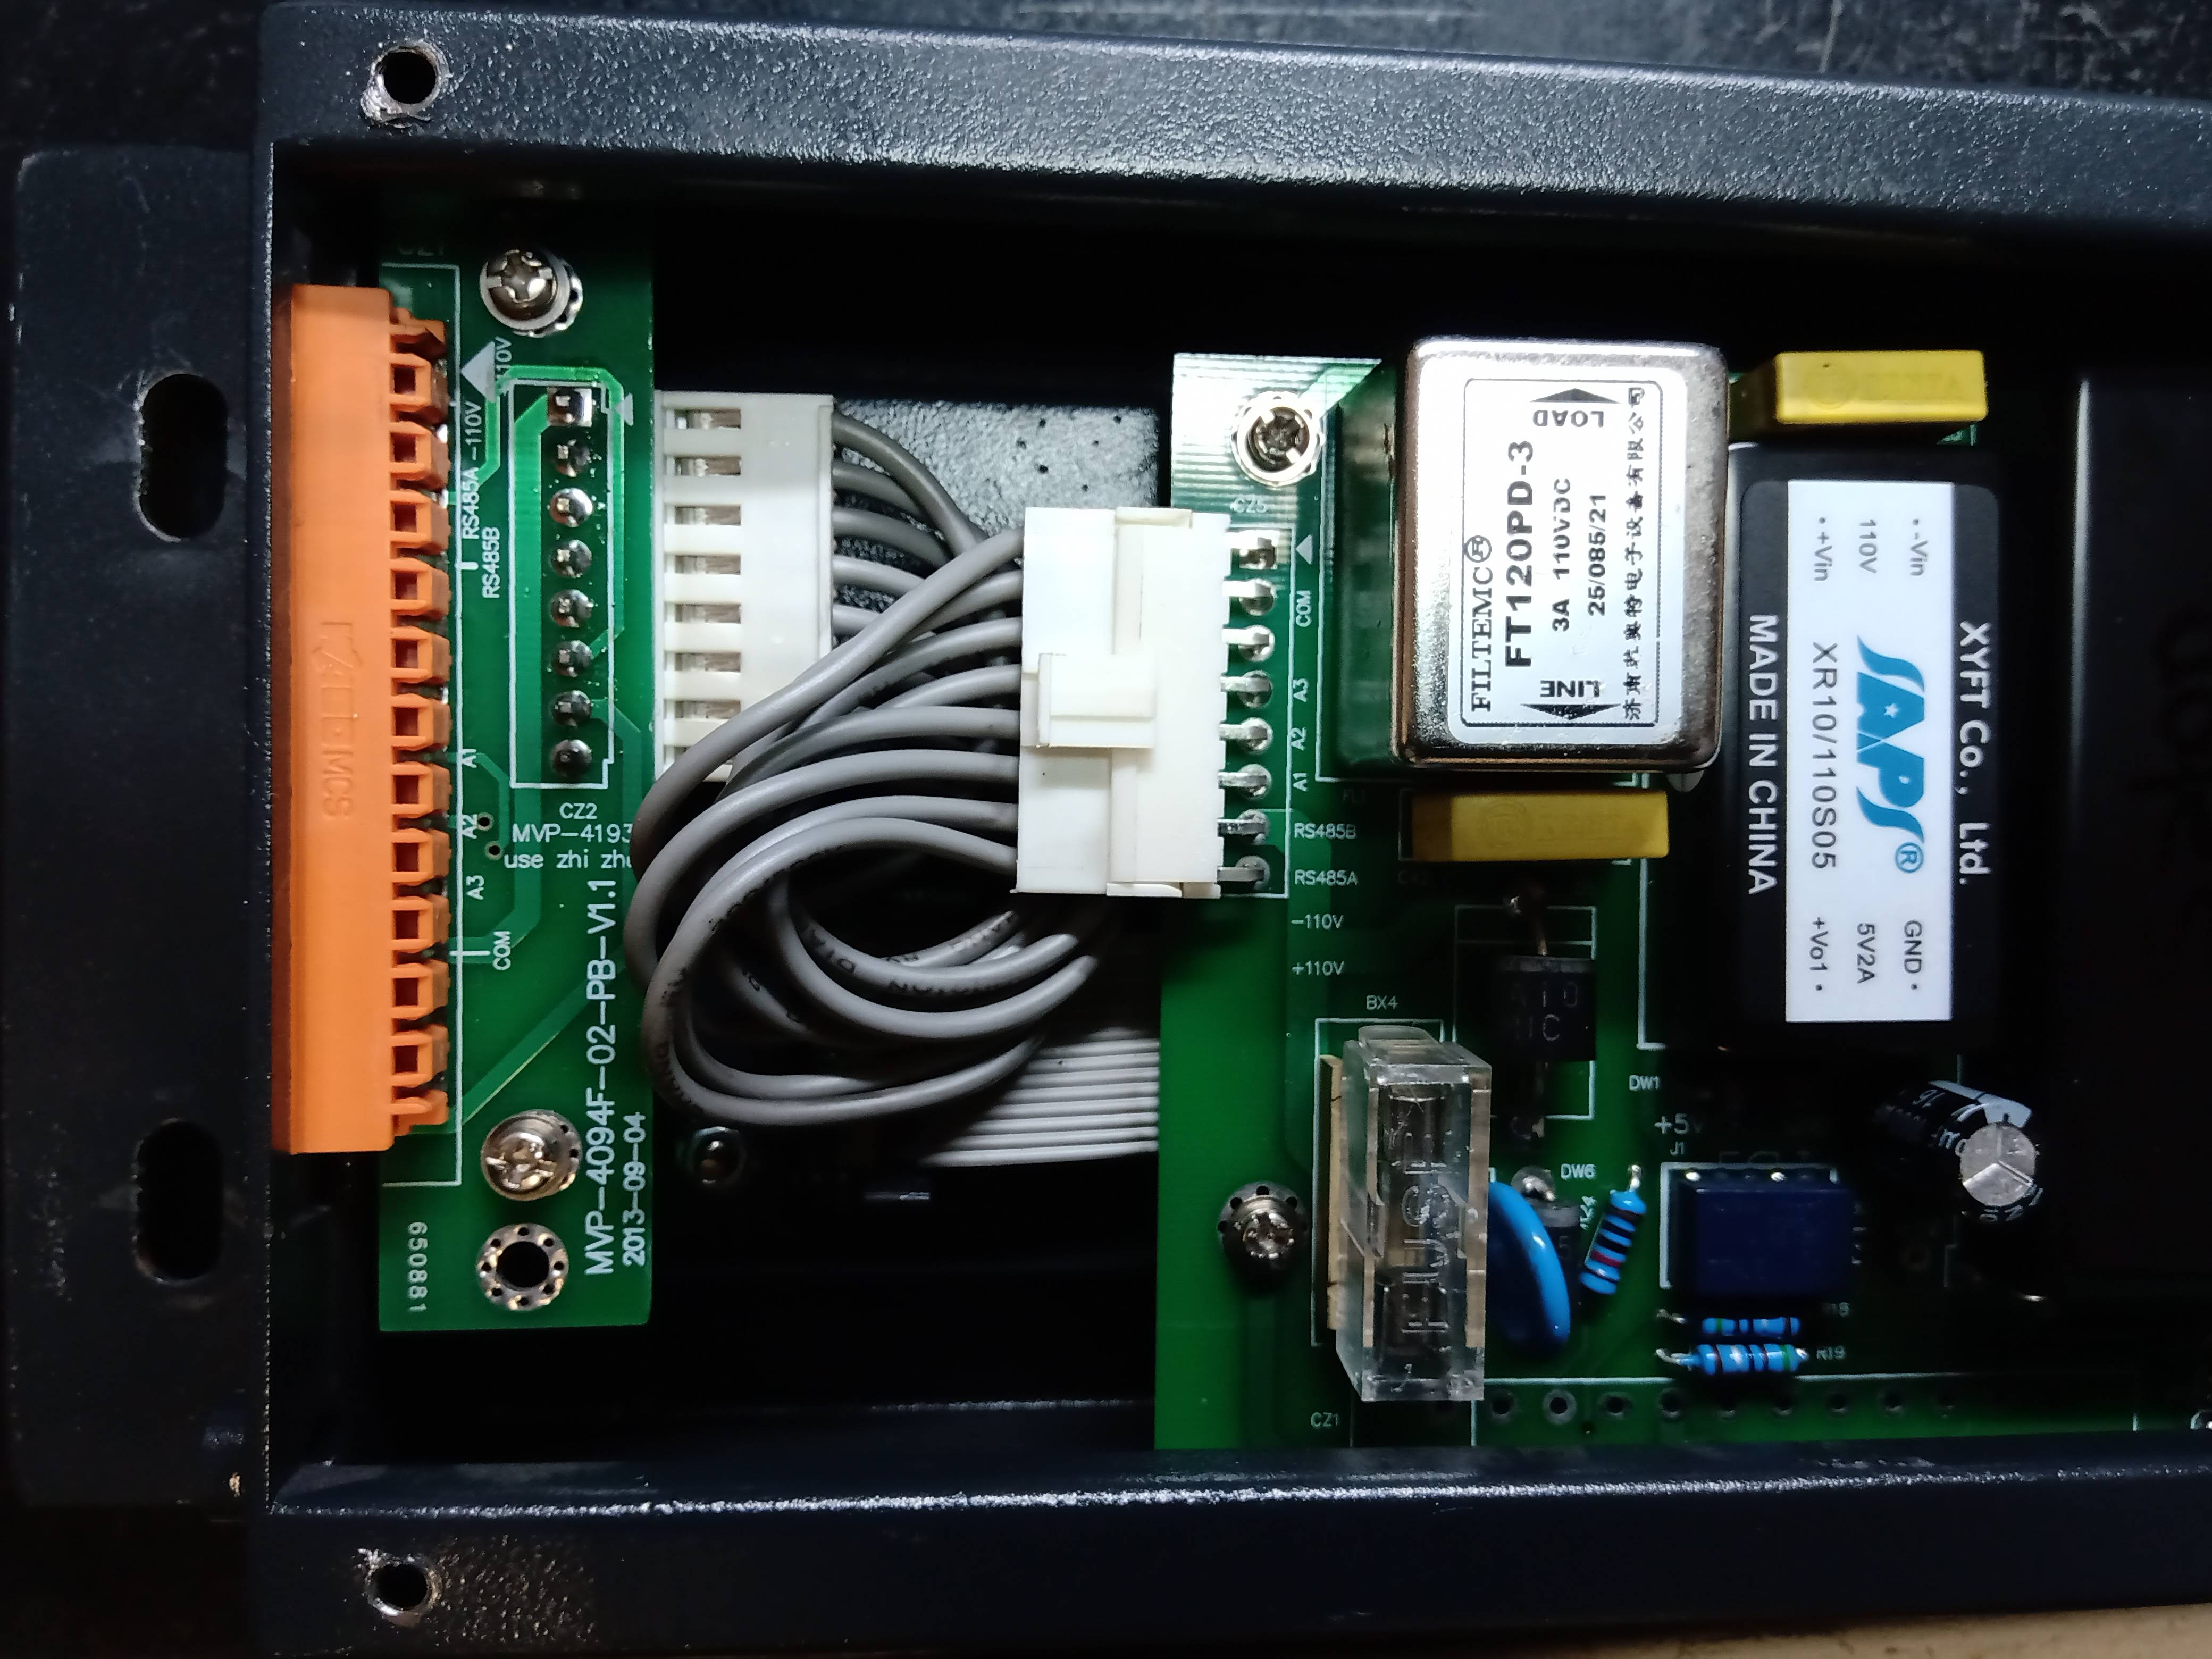
\includegraphics[width=0.75\textwidth]{./Figures/displayController.jpg}
	\caption{Fotografía del detalle de conexión de la placa de control de los carteles led de salón.}
	\label{fig:displayController}
\end{figure}


\begin{figure}[H]
	\centering
	\includegraphics[width=0.5\textwidth, angle=90]{./Figures/placaIDU.jpg}
	\caption{Placa de control (IDU) de los carteles de matriz led.}
	\label{fig:placa}
\end{figure}

\begin{figure}[H]
	\centering
	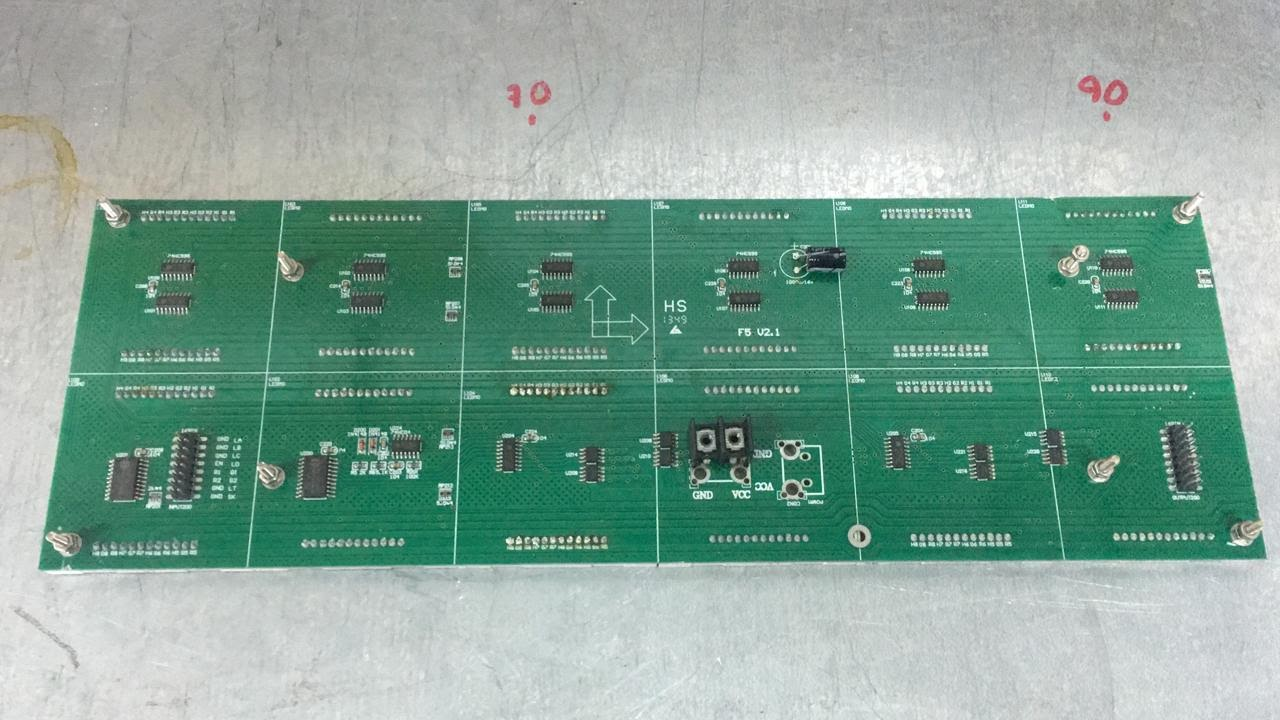
\includegraphics[width=1\textwidth]{./Figures/cartel2x6.jpeg}
	\caption{Placa de los carteles de matriz led.}
	\label{fig:placaDisplay}
\end{figure}


\begin{figure}[H]
	\centering
	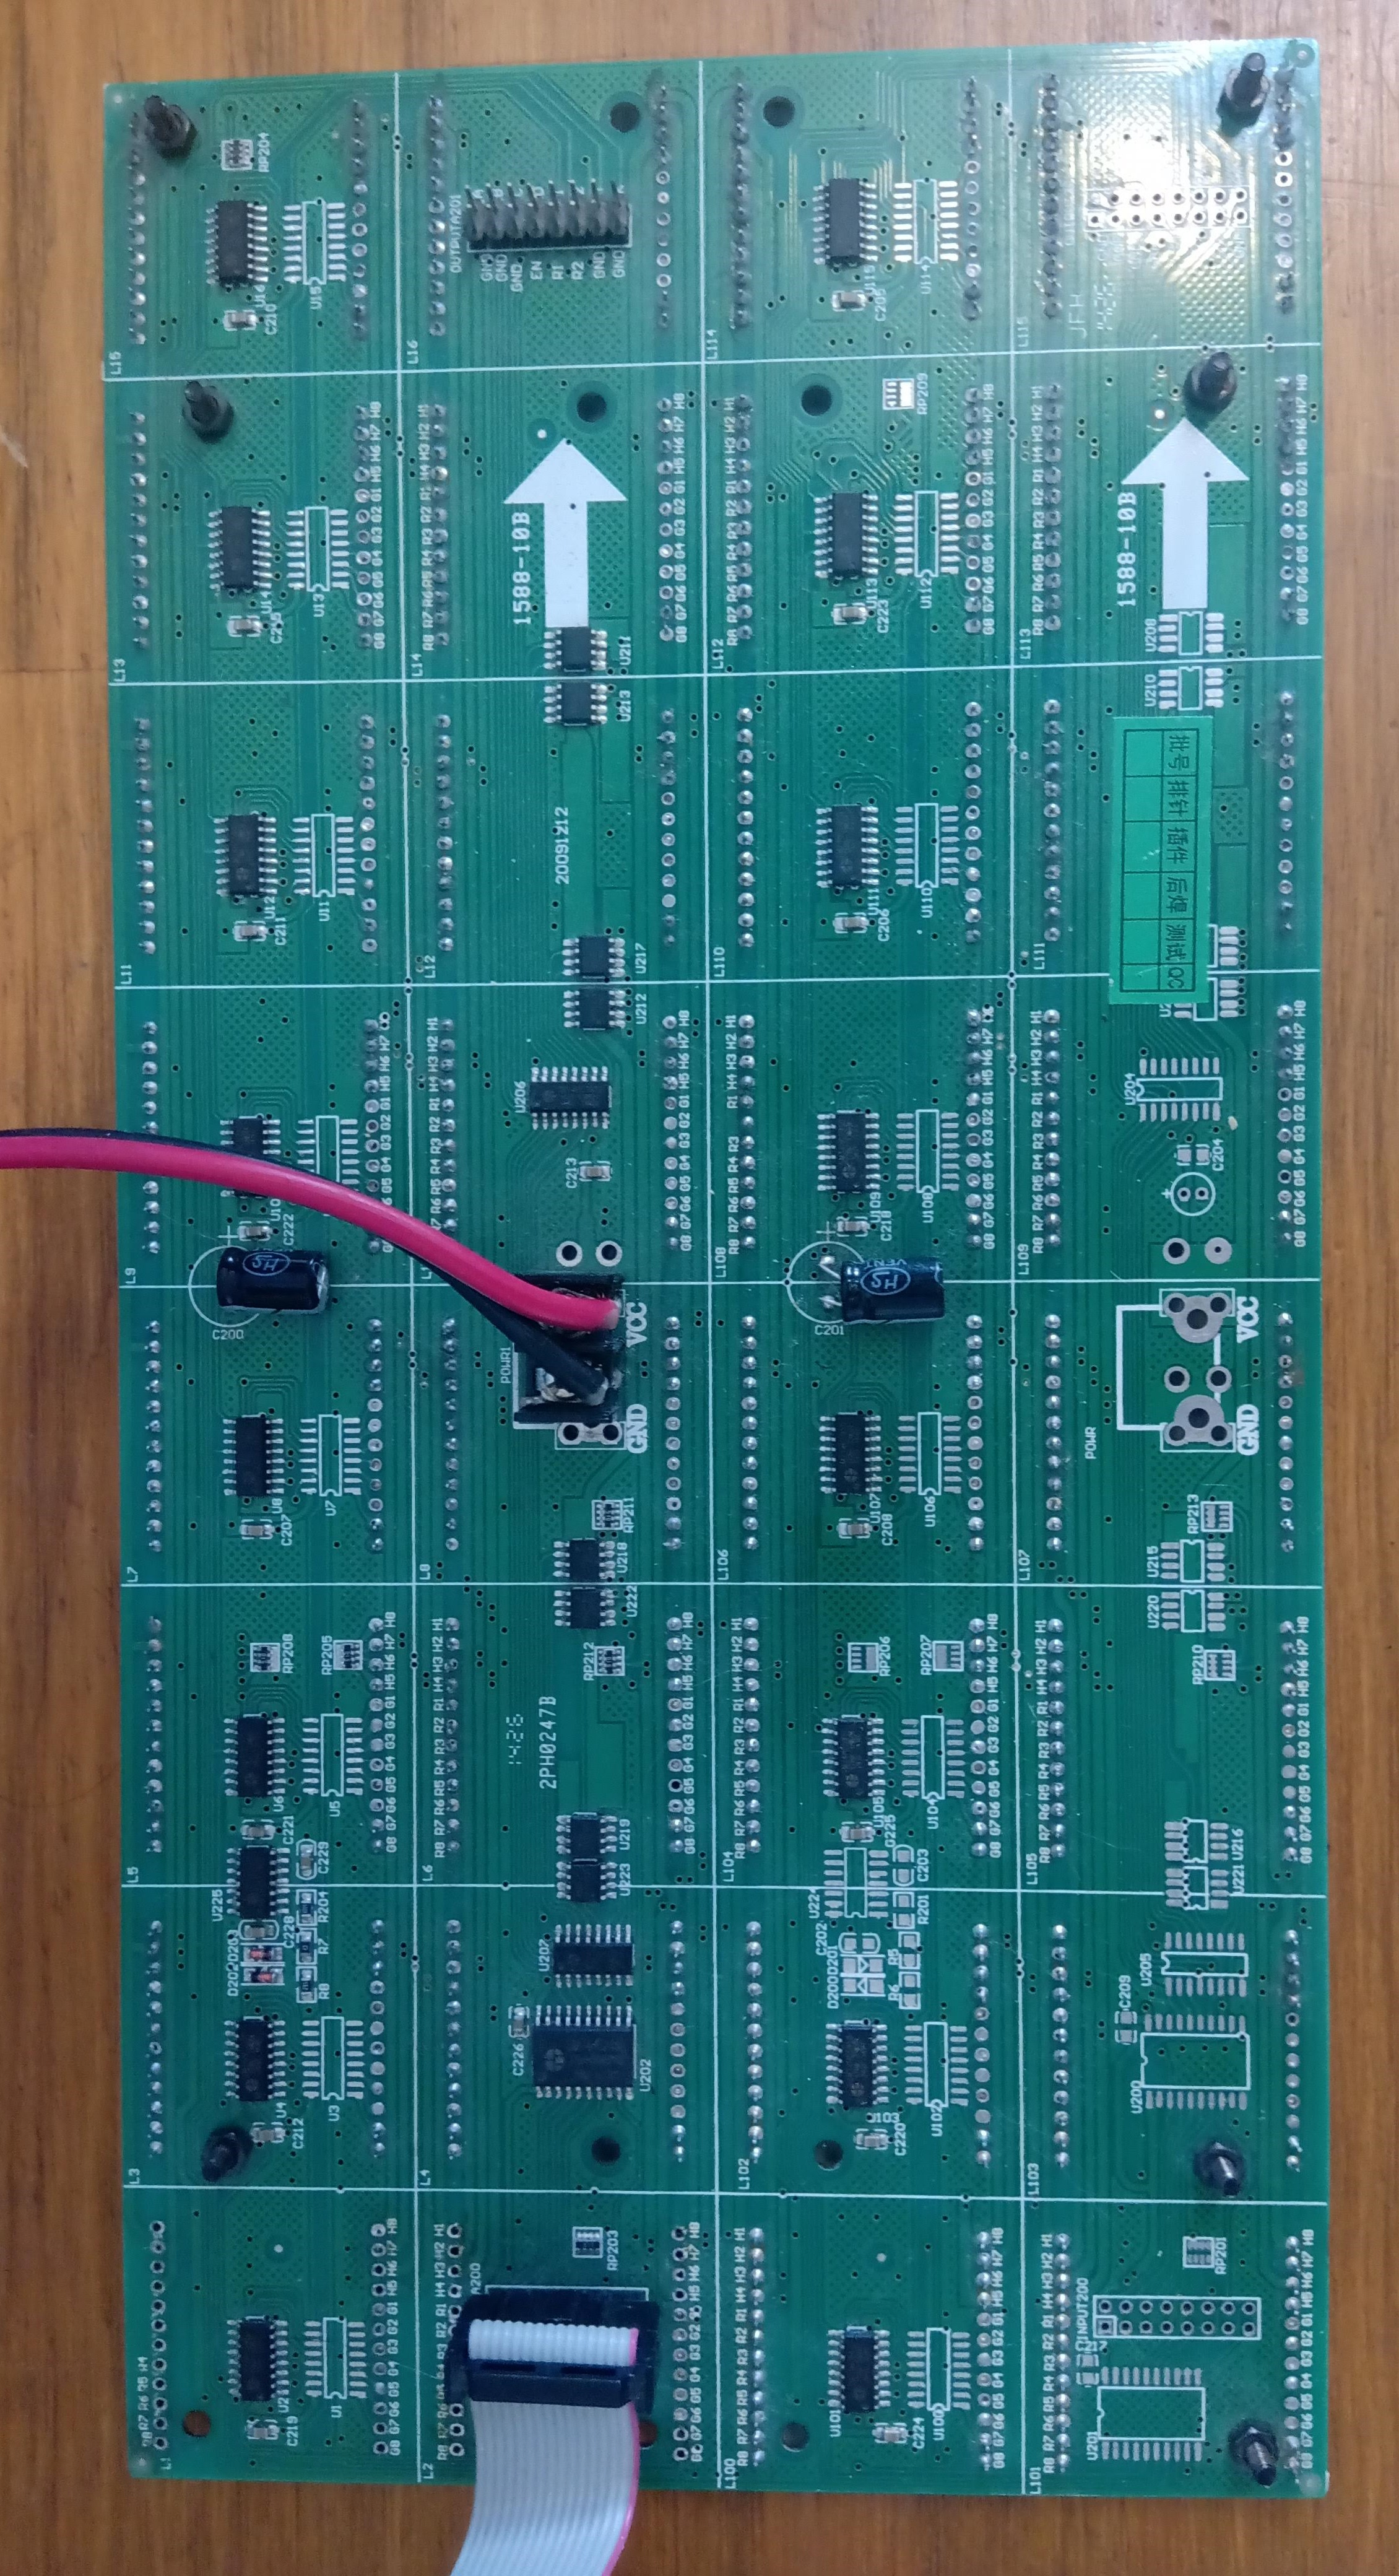
\includegraphics[width=0.75\textwidth, angle=270]{./Figures/cartel4x8.jpg}\\
	\includegraphics[width=1\textwidth]{./Figures/cartelledON.jpg}\\
	\caption{Fotografías de placas de control de los carteles de matriz led: (a) placa de 2x6 módulos; (b) placa de 4x8 módulos; (c) vista posterior de la placa de 4x8.}
	\label{fig:picsDriverled}
\end{figure}


En el circuito esquemático de la figura \ref{fig:schDriverled} se presenta el detalle de conexiones eléctricas entre bloques. Se puede observar que a la salida del conector de datos (CONN 2x8) hay dos buffers de la serie 74HC245D que direccionan las señales eléctricas a izquierda y derecha del arreglo de matrices led. A izquierda viajan las señales SER(data), SRCLK (Clock) y XXX (latch) al arreglo de Shift Registers de la serie 74HC595. Por la derecha se maneja la habilitación secuencial de las filas a través de un arreglo de decodificadores 3x8 de la serie 74HC138. Cada salida de los decodificadores se conecta a un driver de corriente en arreglo de transistores MOSFET FDS4953. Estos decodificadores cableados adecuadamente permiten manejar las 32 señales de un cartel de 4x8 módulos led. \\

\section{Pruebas realizadas}

\pagebreak

\section{APÉNDICE}


\begin{figure}[H]
	\centering
	%\includepdf[pages={1}, angle=90]{./Figures/output.driverled.pdf}
	\includegraphics[width=1.66\textwidth, angle=90]{./Figures/output.driverled.pdf}
	\caption{Circuito esquemático de la placa controladora de los carteles de matriz led.}
	\label{fig:schDriverled}
\end{figure}

\begin{figure}[H]
	\centering
	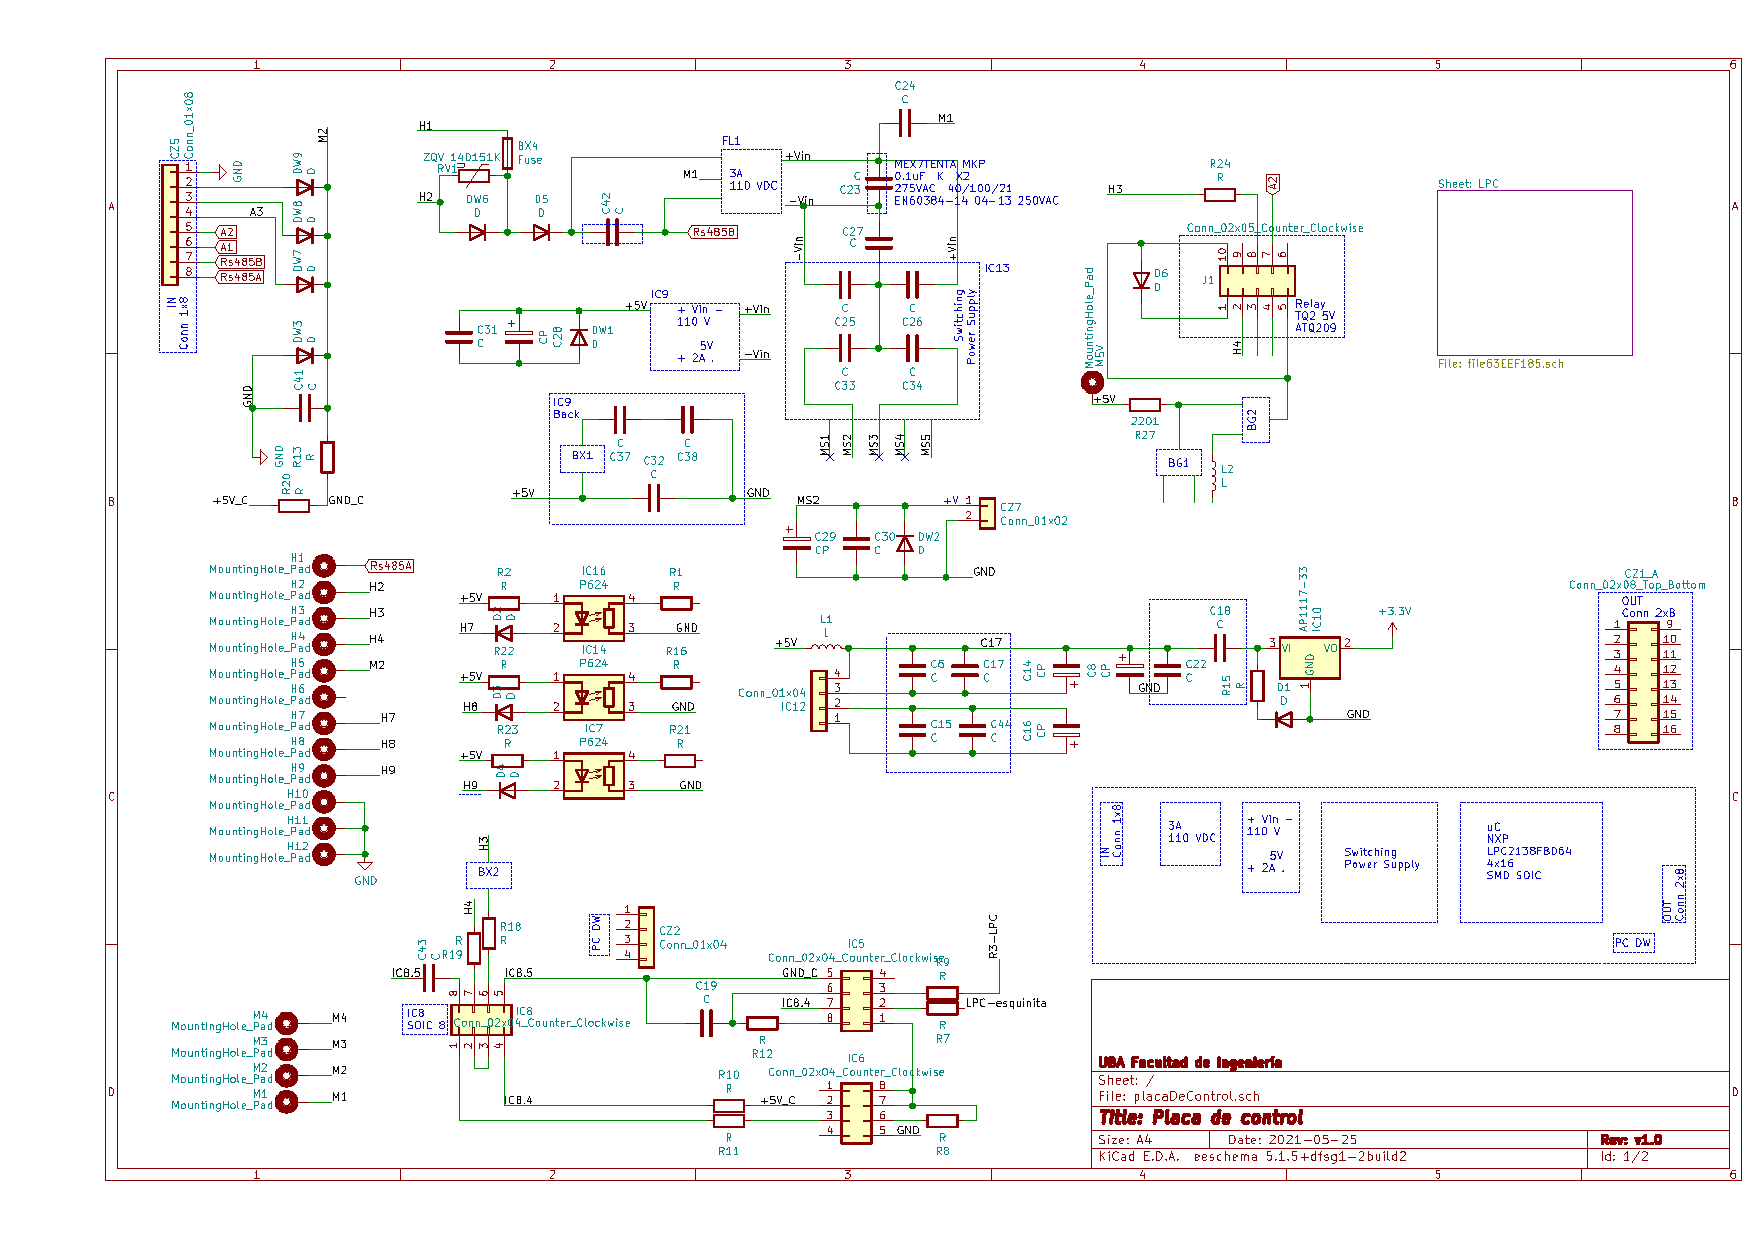
\includegraphics[width=1.66\textwidth, angle=90]{./Figures/output.placaControl.pdf}
	\caption{Circuito esquemático de la placa de control de los carteles LED de salón.}
	\label{fig:schController}
\end{figure}